\section{Tip Selection}\label{tip-selection}

Unapproved transactions are called tips. This section covers the reasons why the process of selecting a tip is important for the network.
In order to discuss the tip selection algorithm, a simulation of the DAG architecture is characterized by the following two parameters. 


\begin{description}
    \item[Transaction rate $\bm{\lambda}$] Transactions do not arrive evenly throughout time. To model such behaviour, a mathematical object called Poisson point process is used. The arrival rate of transactions is specified by the parameter $\lambda$. The higher $\lambda$ is set in the simulation, the more transactions arrive within one time-unit. If $\lambda$ is set to a really small number, the graph grows in the form of a linked list as there is always just one tip to be approved by a new transaction. Figure \ref{fig:simulation} shows a simulation, where $\lambda=5$. The tips are drawn as grey boxes.
    \item[Delay $\bm{h}$] As new transactions must perform computational work for spam prevention and this computation is based on the selected tip of that transactions, there is a delay between choosing the tips and publishing the transaction. This delay is defined by the parameter $h$. For a device with less computational power, $h$ will be larger than for computers with higher processing power. The simulation in Figure \ref{fig:simulation} assumes that $d=1$ for every device that adds a new transaction. Thus, for example the node issuing transaction 5 did not know about the transactions 1-4 when he started with the PoW computation for transaction 5. The time difference to transactions 1-4 is less than $d$. 
\end{description}

\begin{figure}[H]
    \centering
    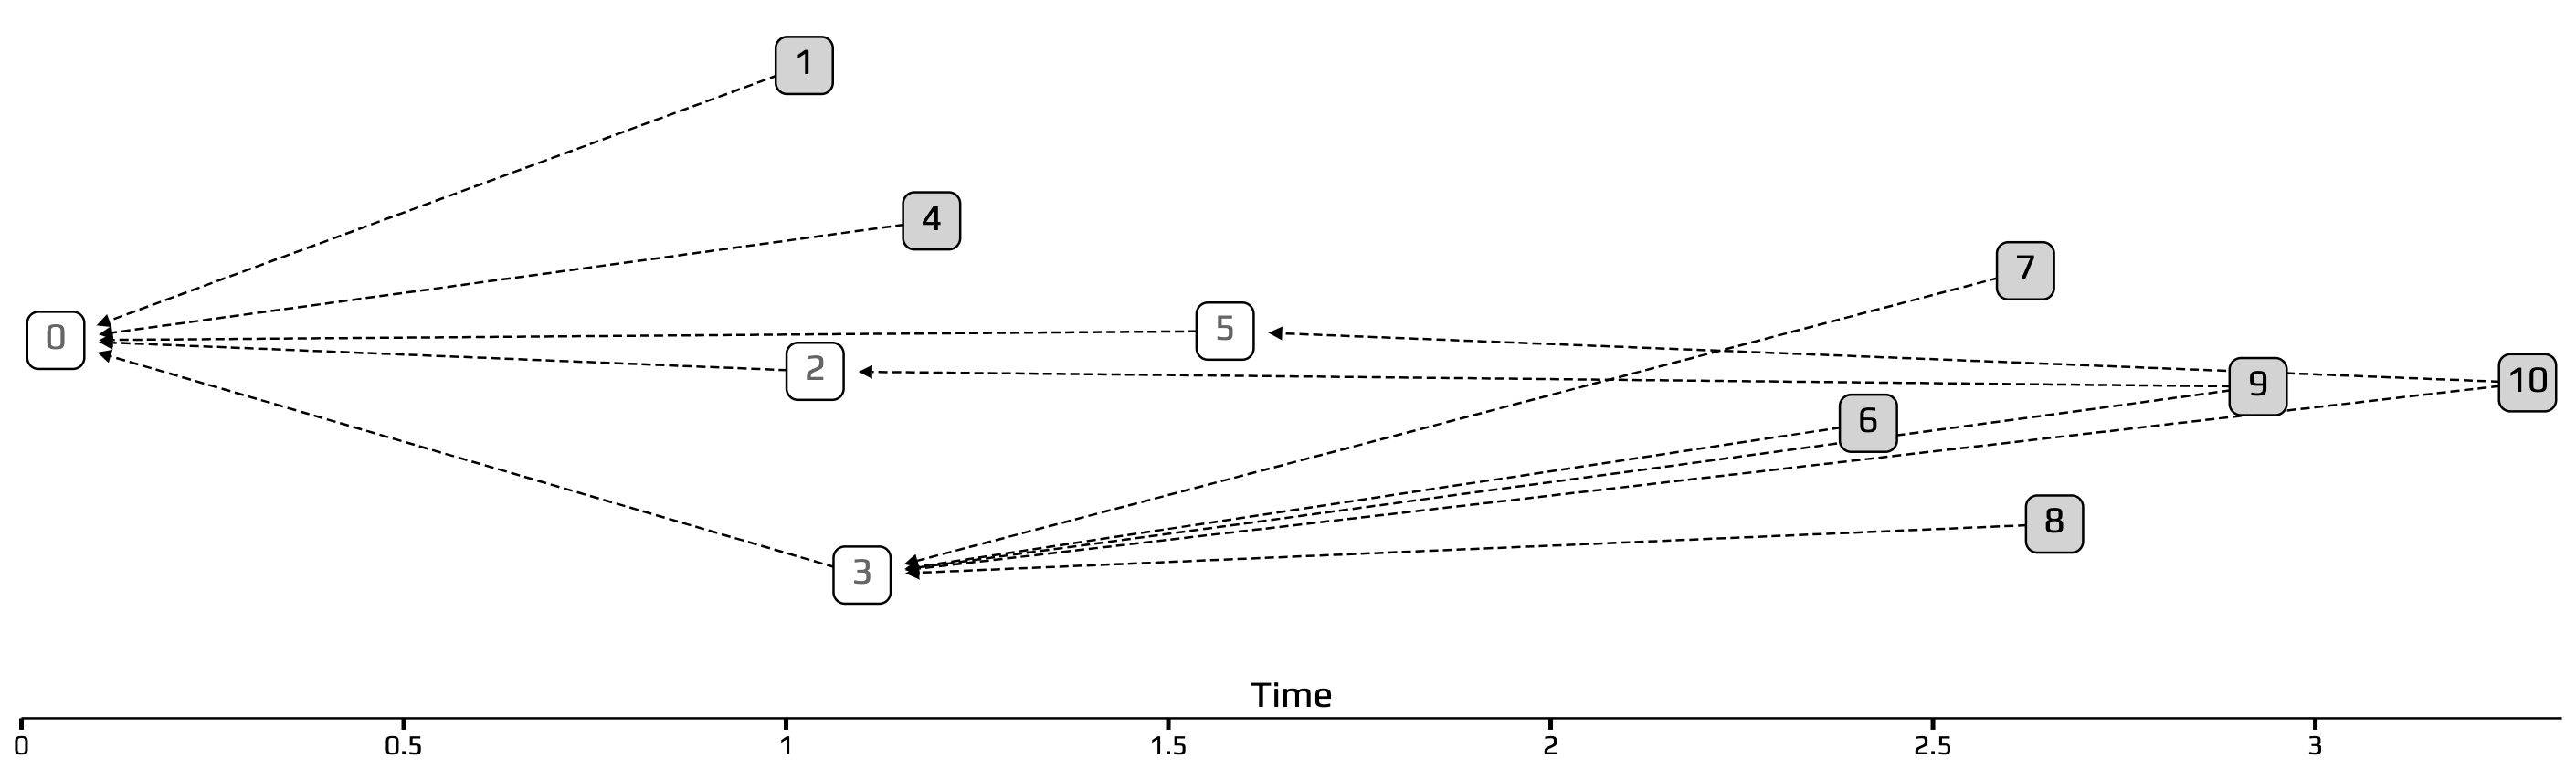
\includegraphics[width=1.0\textwidth]{images/simulation.png}
    \caption{Simulation with $\lambda=5$ and $d=1$  \cite{the-tangle-part-3}}
    \label{fig:simulation}
\end{figure}


There is a possibility that one or both of the validated transactions might no longer be a tip at the time of broadcasting the new transaction. Thus, the tangle must also accept transactions that approve already verified transactions. However, the tip selection algorithm must avoid these \textit{lazy tips} which point to older transactions. Confirming old transaction is unwanted since it increases the branching factor of the graph and thus, it increases the number of tips. Furthermore, \textit{lazy} nodes do not help the network to grow since no unapproved transactions are confirmed. In Figure \ref{fig:lazy-tip}, transaction 14 is added to the network by a lazy node. 


\begin{figure}[H]
    \centering
    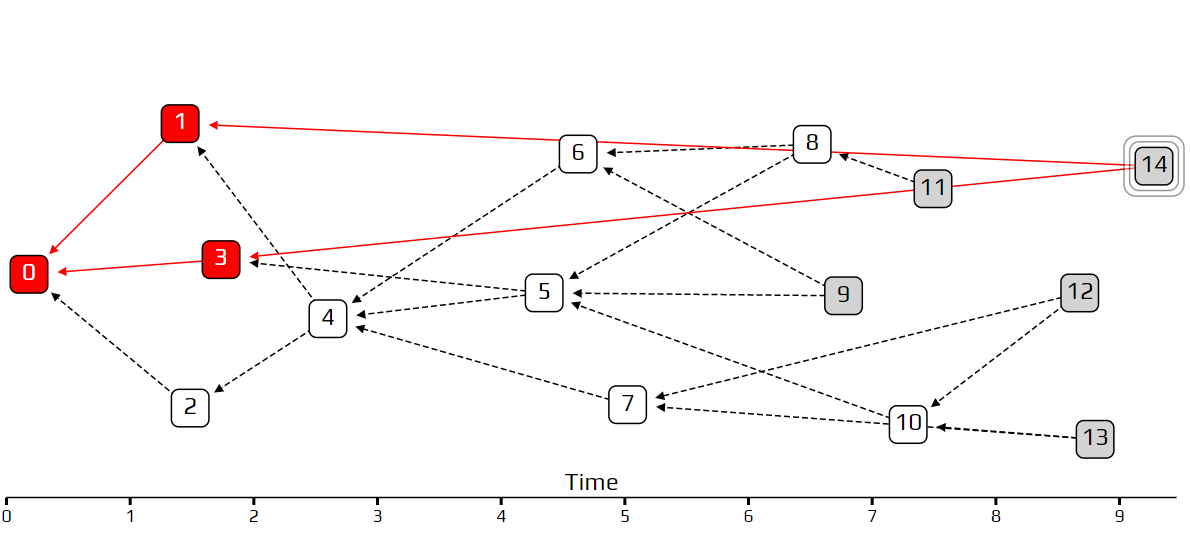
\includegraphics[width=1.0\textwidth]{images/lazy-tip.png}
    \caption{Lazy Tip \cite{the-tangle-part-3}}
    \label{fig:lazy-tip}
\end{figure}

For finding a tip, a node must walk from the genesis until it reaches an unconfirmed transaction. The node has to choose between multiple possible paths. If the node chooses the path solely based on the branching factor, transactions added by lazy nodes would be selected with the same probability as any other transaction. Thus, the random walk algorithm must be less biased towards lazy transactions. 
This is achieved by favoring transactions that have a higher cumulative weight. The bias factor is defined with the parameter $\alpha$. Setting $\alpha$ to a high value results in many unconfirmed transactions since most approvers choose the same path to the tip. These unconfirmed transactions are left behind and will never be accepted. Thus, determining an ideal value for $\alpha$ is crucial for the usability of the network and depends on the transaction arrival rate, the PoW delay of different devices in the network, network delay and the number of tips. 

The method of setting a rule on how to find a path towards a tip is called a Markov Chain Monte Carlo technique (MCMC) \cite{mcmc}. In a Markov chain, each step enforces a rule which is defined in advanced and does not depend on the previous step. In the example of the Tangle, each step is a node in the graph and the rules are the probabilities of the available paths depending on the cumulative weights.

Figure \ref{fig:mcmc} illustrates the simulation of a random walk algorithm. It is assumed that the network delay is 1 time unit. Thus, the node that issues transaction 9 does not know about transaction 7 and 8. As transaciton 6 confirms transaction 1, transaction 1 has a cumulative weight of 2. Therefore, it is more likely to choose the path with a higher cumulative weight.

\begin{figure}[H]
    \centering
    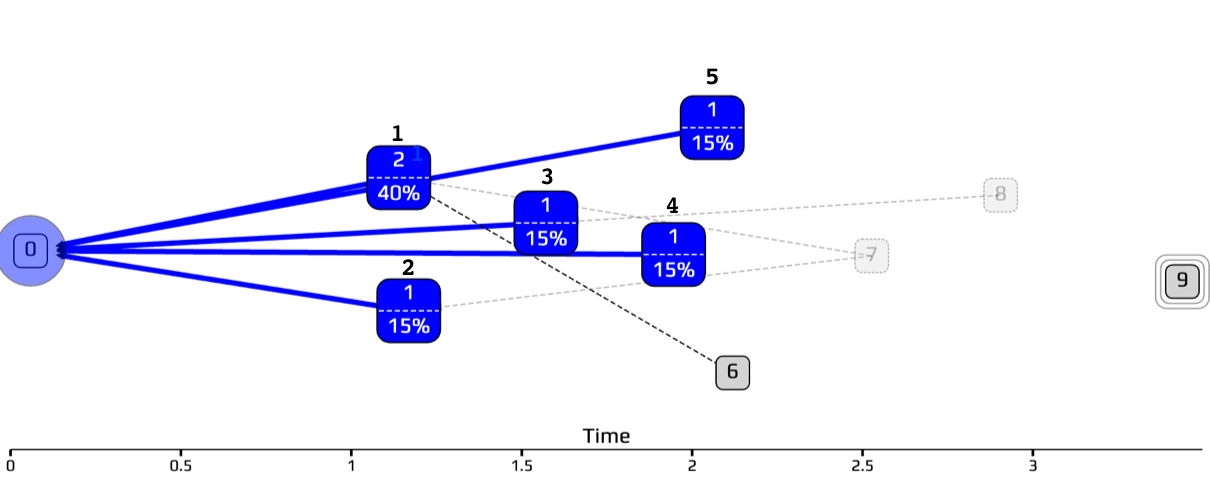
\includegraphics[width=1.0\textwidth]{images/mcmc.png}
    \caption{Markov Chain Monte Carlo Technique}
    \label{fig:mcmc}
\end{figure}